
\let\negmedspace\undefined
\let\negthickspace\undefined
\documentclass[journal,12pt,onecolumn]{IEEEtran}
\usepackage{setspace}
\singlespacing
\usepackage{tikz}
\usetikzlibrary{shapes, arrows}
\usepackage[cmex10]{amsmath}
\usepackage{amsthm}
\usepackage{mathrsfs}
\usepackage{txfonts}
\usepackage{stfloats}
\usepackage{floatrow}
\usepackage{bm}
\usepackage{cite}
\usepackage{cases}
\usepackage{subfig}
\usepackage{longtable}
\usepackage{multirow}
\usepackage{enumitem}
\usepackage{mathtools}
\usepackage{tikz}
\usepackage{circuitikz}
\usepackage{verbatim}
\usepackage[breaklinks=true]{hyperref}
\usepackage{tkz-euclide} % loads  TikZ and tkz-base
\usepackage{listings}
\usepackage{color}    
\usepackage{array}    
\usepackage{longtable}
\usepackage{calc}     
\usepackage{multirow} 
\usepackage{hhline}   
\usepackage{ifthen}   
\usepackage{lscape}     
\usepackage{chngcntr}
\DeclareMathOperator*{\Res}{Res}
\renewcommand\thesection{\arabic{section}}
\renewcommand\thesubsection{\thesection.\arabic{subsection}}
\renewcommand\thesubsubsection{\thesubsection.\arabic{subsubsection}}
\renewcommand\thesectiondis{\arabic{section}}
\renewcommand\thesubsectiondis{\thesectiondis.\arabic{subsection}}
\renewcommand\thesubsubsectiondis{\thesubsectiondis.\arabic{subsubsection}}
\renewcommand{\thefigure}{\theenumi}
\renewcommand{\thetable}{\theenumi}
\providecommand{\gauss}[2]{\mathcal{N}\ensuremath{\left(#1,#2\right)}}
% correct bad hyphenation here
\hyphenation{op-tical net-works semi-conduc-tor}
\def\inputGnumericTable{}                                 %%

\lstset{
%language=C,
frame=single, 
breaklines=true,
columns=fullflexible
}
%\lstset{
%language=tex,
%frame=single, 
%breaklines=true
%}
\begin{document}
\newtheorem{theorem}{Theorem}[section]
\newtheorem{problem}{Problem}
\newtheorem{proposition}{Proposition}[section]
\newtheorem{lemma}{Lemma}[section]
\newtheorem{corollary}[theorem]{Corollary}
\newtheorem{example}{Example}[section]
\newtheorem{definition}[problem]{Definition}
\newcommand{\BEQA}{\begin{eqnarray}}
\newcommand{\EEQA}{\end{eqnarray}}
\newcommand{\define}{\stackrel{\triangle}{=}}
\bibliographystyle{IEEEtran}
\providecommand{\mbf}{\mathbf}
\providecommand{\pr}[1]{\ensuremath{\Pr\left(#1\right)}}
\providecommand{\qfunc}[1]{\ensuremath{Q\left(#1\right)}}
\providecommand{\sbrak}[1]{\ensuremath{{}\left[#1\right]}}
\providecommand{\lsbrak}[1]{\ensuremath{{}\left[#1\right.}}
\providecommand{\rsbrak}[1]{\ensuremath{{}\left.#1\right]}}
\providecommand{\brak}[1]{\ensuremath{\left(#1\right)}}
\providecommand{\lbrak}[1]{\ensuremath{\left(#1\right.}}
\providecommand{\rbrak}[1]{\ensuremath{\left.#1\right)}}
\providecommand{\cbrak}[1]{\ensuremath{\left\{#1\right\}}}
\providecommand{\lcbrak}[1]{\ensuremath{\left\{#1\right.}}
\providecommand{\rcbrak}[1]{\ensuremath{\left.#1\right\}}}
\theoremstyle{remark}
\newtheorem{rem}{Remark}
\newcommand{\sgn}{\mathop{\mathrm{sgn}}}
\providecommand{\abs}[1]{\left\vert#1\right\vert}
\providecommand{\res}[1]{\Res\displaylimits_{#1}} 
\providecommand{\norm}[1]{\left\lVert#1\right\rVert}
\providecommand{\mtx}[1]{\mathbf{#1}}
\providecommand{\mean}[1]{E\left[ #1 \right]}
\providecommand{\fourier}{\overset{\mathcal{F}}{ \rightleftharpoons}}
\providecommand{\system}[1]{\overset{\mathcal{#1}}{ \longleftrightarrow}}
\newcommand{\solution}{\noindent \textbf{Solution: }}
\newcommand{\cosec}{\,\text{cosec}\,}
\providecommand{\dec}[2]{\ensuremath{\overset{#1}{\underset{#2}{\gtrless}}}}
\newcommand{\myvec}[1]{\ensuremath{\begin{pmatrix}#1\end{pmatrix}}}
\newcommand{\mydet}[1]{\ensuremath{\begin{vmatrix}#1\end{vmatrix}}}
\let\vec\mathbf
\def\putbox#1#2#3{\makebox[0in][l]{\makebox[#1][l]{}\raisebox{\baselineskip}[0in][0in]{\raisebox{#2}[0in][0in]{#3}}}}
     \def\rightbox#1{\makebox[0in][r]{#1}}
     \def\centbox#1{\makebox[0in]{#1}}
     \def\topbox#1{\raisebox{-\baselineskip}[0in][0in]{#1}}
     \def\midbox#1{\raisebox{-0.5\baselineskip}[0in][0in]{#1}}
\setlength{\parindent}{0pt}
\bibliographystyle{IEEEtran}
\newenvironment{amatrix}[1]{%
  \left(\begin{array}{@{}*{#1}{c}|c@{}}
}{%
  \end{array}\right)
}
\title{
%	\logo{
GATE BM 2023 Quetion 9
%	}
}
\author{ Snehil Singh EE22BTECH11050$^{*}$% <-this % stops a space
	%
}
	
	
%\title{
%	\logo{Matrix Analysis through Octave}{\begin{center}\includegraphics[scale=.24]{tlc}\end{center}}{}{HAMDSP}
%}


% paper title
% can use linebreaks \\ within to get better formatting as desired
%\title{Matrix Analysis through Octave}
%
%
% author names and IEEE memberships
% note positions of commas and nonbreaking spaces ( ~ ) LaTeX will not break
% a structure at a ~ so this keeps an author's name from being broken across
% two lines.
% use \thanks{} to gain access to the first footnote area
% a separate \thanks must be used for each paragraph as LaTeX2e's \thanks
% was not built to handle multiple paragraphs
%
%\author{<-this % stops a space
%\thanks{}}
%}
% note the % following the last \IEEEmembership and also \thanks - 
% these prevent an unwanted space from occurring between the last author name
% and the end of the author line. i.e., if you had this:
% 
% \author{....lastname \thanks{...} \thanks{...} }
%                     ^------------^------------^----Do not want these spaces!
%
% a space would be appended to the last name and could cause every name on that
% line to be shifted left slightly. This is one of those "LaTeX things". For
% instance, "\textbf{A} \textbf{B}" will typeset as "A B" not "AB". To get
% "AB" then you have to do: "\textbf{A}\textbf{B}"
% \thanks is no different in this regard, so shield the last } of each \thanks
% that ends a line with a % and do not let a space in before the next \thanks.
% Spaces after \IEEEmembership other than the last one are OK (and needed) as
% you are supposed to have spaces between the names. For what it is worth,
% this is a minor point as most people would not even notice if the said evil
% space somehow managed to creep in.



% The paper headers
%\markboth{Journal of \LaTeX\ Class Files,~Vol.~6, No.~1, January~2007}%
%{Shell \MakeLowercase{\textit{et al.}}: Bare Demo of IEEEtran.cls for Journals}
% The only time the second header will appear is for the odd numbered pages
% after the title page when using the twoside option.
% 
% *** Note that you probably will NOT want to include the author's ***
% *** name in the headers of peer review papers.                   ***
% You can use \ifCLASSOPTIONpeerreview for conditional compilation here if
% you desire.




% If you want to put a publisher's ID mark on the page you can do it like
% this:
%\IEEEpubid{0000--0000/00\$00.00~\copyright~2007 IEEE}
% Remember, if you use this you must call \IEEEpubidadjcol in the second
% column for its text to clear the IEEEpubid mark.
% make the title area 
\maketitle


%\tableofcontents

\bigskip

\renewcommand{\thefigure}{\arabic{figure}}
\renewcommand{\thetable}{\theenumi}
%\renewcommand{\theequation}{\theenumi}

%\begin{abstract}
%%\boldmath
%In this letter, an algorithm for evaluating the exact analytical bit error rate  (BER)  for the piecewise linear (PL) combiner for  multiple relays is presented. Previous results were available only for upto three relays. The algorithm is unique in the sense that  the actual mathematical expressions, that are prohibitively large, need not be explicitly obtained. The diversity gain due to multiple relays is shown through plots of the analytical BER, well supported by simulations. 
%
%\end{abstract}
% IEEEtran.cls defaults to using nonbold math in the Abstract.
% This preserves the distinction between vectors and scalars. However,
% if the journal you are submitting to favors bold math in the abstract,
% then you can use LaTeX's standard command \boldmath at the very start
% of the abstract to achieve this. Many IEEE journals frown on math
% in the abstract anyway.

% Note that keywords are not normally used for peerreview papers.
%\begin{IEEEkeywords}
%Cooperative diversity, decode and forward, piecewise linear
%\end{IEEEkeywords} 
\textbf{Question :}\\
Out of 1000 individuals in a town, 100 unidentified individuals are covid positive.
Due to lack of adequate covid-testing kits, the health authorities of the town devised
a strategy to identify these covid-positive individuals. The strategy is to:
\begin{enumerate}
\item Collect saliva samples from all 1000 individuals and randomly group
them into sets of 5.
\item Mix the samples within each set and test the mixed sample for covid.
\item If the test done in (ii) gives a negative result, then declare all the 5
individuals to be covid negative.
\item If the test done in (ii) gives a positive result, then all the 5 individuals
are separately tested for covid.
\end{enumerate}
Given this strategy, no more than testing kits will be required to identify
all the 100 covid positive individuals irrespective of how they are grouped \\ 
\begin{enumerate}
\item 700
\item 600
\item 800
\item 1000
\end{enumerate}

\textbf{Solution :}


Given : \\
\begin{table}[H]
\def\arraystretch{1.2}
\begin{tabular}{|c|c|}
\hline
	\textbf{Parameter} &\textbf{Value} \\ \hline
	Number of individuals &1000 \\ \hline
	Strength of each group &5 \\ 
	\hline
	Number of groups &200 \\ 
	\hline
	Number of Covid positive individuals &100 \\ \hline
	
	
\end{tabular}
\end{table}
At first we ll have to examine all the groups and then test all 5 individuals of each group who tested positive.\\ \\
Using binomial expansion to find the probability of a group testing positive \\
\begin{table}[H]
\def\arraystretch{1.2}
\begin{tabular}{|c|c|c|}
\hline
	\textbf{Parameter} &\textbf{Value} &\textbf{Expression} \\ \hline
	N &1000 &Total number of individuals \\ \hline
	n &5 &Number of individuals in group \\ \hline
	p &0.1 &Probability of individual testing positive \\ \hline
	q &0.9 &Probability of individual testing negative \\ \hline	
\end{tabular}
\end{table}
Probability of a group of 5 with i covid negative individuals is given as \\
the PMF:
\begin{align}
Pr(X=i) &= ^{n}C_{i}(q)^{i}(p)^{n-i} \\
&= ^{5}C_{i}(0.9)^{i}(0.1)^{5-i}
\end{align}
Let us assume X is a random variable which denotes the number of individuals tested negative in a group.
Probability of group having atmost k negative tested individuals \\
the CDF :
\begin{align}
F_{X}(k) &= Pr(X \le k) \\
&= \Sigma_{i=0}^k ^{n}C_{i}(q)^{i}(p)^{n-i} \\
&= \Sigma_{i=0}^k ^{5}C_{i}(0.9)^{i}(0.1)^{5-i} \\
\end{align}
If a group is tested positive, atleast one of the 5 individuals should be covid positive which means atmost 4 individuals are covid negative. \\
Finding probability of a group testing positive}
\begin{align}
Pr &= F_{X}(4) \\ 
&= \Sigma_{i=0}^4 ^{5}C_{i}(0.9)^{i}(0.1)^{5-i} \\
 &= 0.4096
\end{align}
\begin{table}[H]
\def\arraystretch{1.2}
\begin{tabular}{|c|c|}
\hline
	\textbf{Parameter} &\textbf{Value} \\ \hline

	Number of tests in first round of testing &A \\ 
	\hline
	Number of groups tested positive in first round &b \\ 
	\hline
	Number of tests in second round of testing &B \\ 
	\hline
	Total number of tests in both rounds &T\\ \hline
	
	
\end{tabular}
\end{table}
In the first round we will test all the 200 groups. \\
Number of tests in first round(A) :
\begin{align*}
A = 200
\end{align*}
Out of these 200 tests,assuming the estimated number of groups tested positive is b \\
If a group is tested positive, atleast one of the 5 is covid positive, which impies the group can only have atmost 4 covid negative individual. \\
Calculating b :
\begin{align}
 \text{Pr}(\text{of group testing positive}) &= \frac{b}{A} \\
 F_{X}(4) &= \frac{b}{A}
 \end{align}
 \begin{align}
 \implies b &= 81.92
\end{align}
In all the groups tested positive, atleast one individual is covid positive, to find all the covid positive individuals, we will test all the 5 individuals of the positive groups seperately in round 2. \\
So estimated number tests in round 2 (B) :
\begin{align}
B &= 5b \\ &= \brak{5}\brak{81.92} \\ &= 409.6
\end{align}
Total number of tests estimated (T) :
\begin{align}
T &= A + B \\ &= 200 + 409.6 \\ &= 609.6
\end{align}

$\therefore$ So 609.6 is the expected number of tests required to detect all the covid positive individuals. \\
According to the options, no more than 700 tests will be required.

\textbf{So, the correct answer is option A 700}. \\ \\
\textbf{Simulation :} \\ 
\begin{enumerate}
    \item Including standard C libraries - \texttt{stdio.h} (for input/output), \texttt{stdlib.h} (for dynamic memory allocation), \texttt{time.h} (for time-related functions), and \texttt{math.h} (for mathematical functions). \\
    \item Defining constants for the total number of individuals (\texttt{TOTAL\_INDIVIDUALS}), the number of initially positive individuals (\texttt{POSITIVE\_INDIVIDUALS}), and the group size used in testing (\texttt{GROUP\_SIZE}). \\
    \item Declared a function named \texttt{covidTestingStrategy} that simulates a COVID-19 testing strategy using group testing. The function takes an array of individuals, the total number of individuals, and the number of initially positive individuals as parameters. \\
    \item Initialized variables \texttt{testCount} and \texttt{groupTestTrueCount} to keep track of the total number of tests and the number of group tests that turned out to be true and shuffled the array of individuals randomly using the Fisher-Yates shuffle algorithm to have randomness into the order of testing. \\
    \item We mixed the samples within each group using Bitwise "OR" and tested them.
    \begin{enumerate}
        \item If the mixed sample is negative (\texttt{groupResult == 0}), declares all 5 individuals in the group as COVID negative with one test.
        \item If the mixed sample is positive, tests each individual separately, and increments the test count accordingly.
    \end{enumerate} \\
    \item Calculated the probability of the group test being true based on the initial probability of an individual being positive and the group size and Calculated the expected number of tests for one set, total expected number of sets, and total expected number of tests based on the calculated probabilities. \\
    \item Printed various statistics related to the testing strategy. \\
    \item Seed the random number generator with the current time. Initialized an array representing individuals, marking the first \texttt{POSITIVE\_INDIVIDUALS} as positive. Calls the \texttt{covidTestingStrategy} function with the array and other parameters.
\end{enumerate} \\ \\
Flowchart to explain the function \texttt{covidTestingStrategy} is given below :
\tikzstyle{start} = [ellipse, minimum width=2cm, minimum height=1cm, text centered, draw=black]
\tikzstyle{process} = [rectangle, minimum width=3cm, minimum height=1cm, text centered, draw=black]
\tikzstyle{decision} = [diamond, minimum width=1cm, minimum height=1cm, text centered, draw=black]
\tikzstyle{arrow} = [thick,->,>=stealth]
\tikzstyle{end} = [ellipse, minimum width=2cm, minimum height=1cm, text centered, draw=black]
\begin{center}
\begin{tikzpicture}[node distance=2cm, auto]
  % Nodes
  \node [start] (start) {Start};
  \node [process, below of=start] (initializea) {Initialize Variables and Array};
  \node [process, below of=initializea] (initializeb) {Shuffle the Array};
  \node [process, below of=initializeb] (initializec) {Take samples of groups of 5};
  \node [decision, below of=initializec] (mix) {Test};
  \node [process, below of=mix] (test) {Declare negative};
  \node [end, below of=test] (end1) {End};
  \node [process, right of=mix, xshift=3cm] (testIndividuals) {Test Individuals Separately};
  \node [process, below of=testIndividuals] (incrementCount) {Increment Test Count};
  
 
  \node [process, below of=incrementCount] (calculateProb) {Calculate Probabilities};
  \node [process, below of=calculateProb] (printStats) {Print Statistics};
  \node [end, below of=printStats] (end2) {End};

  % Arrows
  \draw [arrow] (start) -- (initializea);
  \draw [arrow] (initializea) -- (initializeb);
  \draw [arrow] (initializeb) -- (initializec);
  \draw [arrow] (initializec) -- (mix);
  \draw [arrow] (mix) -- (test);
  \draw [arrow] (mix) -- node {Yes} (testIndividuals); 
  \draw [arrow] (mix) -- node {No} (test);
  \draw [arrow] (test) -- (end1);
  \draw [arrow] (testIndividuals) -- (incrementCount);
  \draw [arrow] (incrementCount) -- (calculateProb);
  \draw [arrow] (calculateProb) -- (printStats);
  \draw [arrow] (printStats) -- (end2);
\end{tikzpicture}
\end{center}
\begin{figure}
    \centering
    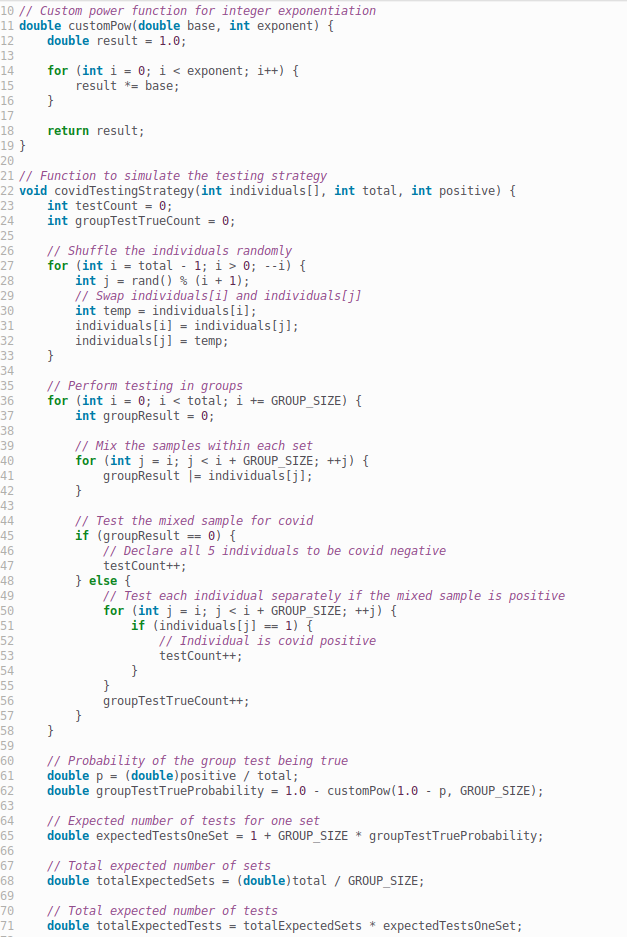
\includegraphics[width=0.8\textwidth]{screenshot/input}
    \caption{Input}
    \label{fig:input}
\end{figure}
\begin{figure}
    \centering
    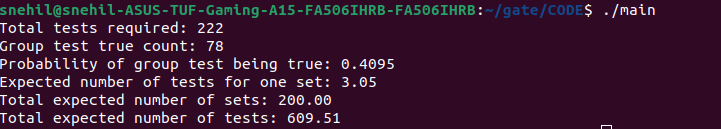
\includegraphics[width=0.8\textwidth]{screenshot/output}
    \caption{Output}
    \label{fig:output}
\end{figure}
\end{document}
